\section{Results \& discussion}

There are separate scripts and Jupyter notebooks for each step of the experimentation available on GitHub\footnote{\href{https://github.com/schmelczer/mir-final}{github.com/schmelczer/mir-final}}. The experiments were run on Leiden University's DS Lab machines. Considering the number of models involved, it took a relatively\footnote{Compared with the amount of time required for pre-training.} short amount of running time to complete: barely over 20 hours on a single GPU.

\subsection{Fine-tuning}

Fine-tuning worked out as expected, all networks were able to find adequately discriminative features. Figure \ref{fig:birds-fine-tuning} and \ref{fig:flowers-fine-tuning} shows the \textit{train} and \textit{validation}\footnote{Which was used to check for overfitting.} accuracies of the image-classification task on the \textit{birds} and \textit{flowers} datasets respectively. Classifying bird species turned out to be significantly more difficult than flowers. In the case of the latter, nearly perfect accuracy is reached, while the best validation accuracy on \textit{birds} is barely over 80\%. In both cases, Inception had the best results, while VGG and ResNet did very similarly. 

The evaluation accuracy seems to be trending upwards even after $20$ epochs, it is likely that better performance could be achieved with longer training, especially, when combined with tuning the learning rate.

\begin{figure*}
  \centering
  \includegraphics[width=1 \linewidth]{figures/birds-finetuning.png}
  \caption{The accuracy metrics over time of the image classifiers on the \textit{birds} train and validation datasets.}
  \label{fig:birds-fine-tuning}
\end{figure*}

\begin{figure*}
  \centering
  \includegraphics[width=1 \linewidth]{figures/flowers-finetuning.png}
  \caption{The accuracy metrics over time of the image classifiers on the \textit{flowers} train and validation datasets.}
  \label{fig:flowers-fine-tuning}
\end{figure*}

\subsection{Results tables}

We have seen that the networks perform reasonably well on their own. When combining them, we get the results of Table \ref{table:birds} and \ref{table:flowers}. The difficulty of \textit{birds} is still clearly visible: the highest Top-1 accuracy on it is achieved by the DistilBERT-VGG pair and is only 19\%, while the Top-5 is 43\%. This duo is strong on \textit{flowers} as well but is very slightly outperformed by DistilBERT-Inception with 40\% and 58\% Top-1 and 5 accuracies respectively. Even though DistilBERT-ResNet never took the first place, its performance is stably the 2\textsuperscript{nd}.

Motivated by the unbalance of \textit{flowers}, an F1 score is included as a metric, however, it does not change the ranking of the models. Also, whichever metric we look at, the pairs with TF-IDF nearly always come last, with the low discriminative power of individual tokens and a tiny dictionary of around 7000 combined with the loss of ordering information are hard to compensate for with another network.

Although the results are ~10\% worse than the best one achieved by Reed et al. \cite{reed2016learning} in their similar setup, it still reveals an interesting potential of this late-fusion architecture: using off-the-shelf networks for highly domain-specific problems is a viable option. It might not result in the best achievable performance --- for that, a custom architecture is likely necessary --- but it is a nearly trivial first approach. For example, it could serve as an ideal baseline model.

\begin{table*}
\def\arraystretch{1.25}
\centering
\caption{Comparison of the 6 presented models on the task of zero-shot text-based image retrieval using the Caltech-UCSD \textit{birds} 200 \cite{welinder2010caltech} dataset.}
\label{table:birds}
\begin{tabular}{|l|r|r|r|r|r|}\hline
    & Top-1 Accuracy & Precision & Recall & F1-score & Top-5 Accuracy \\\hline
   DistilBERT - VGG & 0.19& 0.25& 0.19& 0.19& 0.43\\\hline
   DistilBERT - ResNet & 0.11& 0.17& 0.11& 0.10& 0.32\\\hline
   DistilBERT - Inception v3 & 0.12& 0.33& 0.11& 0.11& 0.29\\\hline
   TF-IDF - VGG & 0.11& 0.28& 0.11& 0.11& 0.33\\\hline
   TF-IDF - ResNet & 0.10& 0.33& 0.10& 0.09& 0.24\\\hline
   TF-IDF - Inception v3 & 0.10& 0.38& 0.10& 0.09& 0.21\\\hline
   \end{tabular}
\end{table*}


\begin{table*}
\vspace{2cm}
\def\arraystretch{1.25}
\centering
\caption{Comparison of the 6 presented models on the task of zero-shot text-based image retrieval using the Oxford-102 \textit{flowers} \cite{Nilsback08} dataset.}
\label{table:flowers}
\begin{tabular}{|l|r|r|r|r|r|}\hline
     & Top-1 Accuracy & Precision & Recall & F1-score & Top-5 Accuracy \\\hline
    DistilBERT - VGG & 0.37& 0.30& 0.27& 0.23& 0.57\\\hline
    DistilBERT - ResNet & 0.36& 0.31& 0.26& 0.24& 0.53\\\hline
    DistilBERT - Inception v3 & 0.40& 0.29& 0.29& 0.27& 0.58\\\hline
    TF-IDF - VGG & 0.20& 0.28& 0.16& 0.13& 0.46\\\hline
    TF-IDF - ResNet & 0.18& 0.28& 0.13& 0.12& 0.33\\\hline
    TF-IDF - Inception v3 & 0.24& 0.24& 0.17& 0.15& 0.43\\\hline
\end{tabular}
\vspace{1.5cm}
\end{table*}

\subsection{Embedding projection}

The aforementioned results are considerably better than random. That means there must be some --- albeit noisy --- transformation between text- and image-embeddings trained using merely semantically similar tasks. Let us investigate them.

Fortunately, with a text embedding size of $l_{text}$ and image embedding size of $l_{image}$ there are only $l_{text} \cdot l_{image}$ weights in the linear projection between them. These are shown in Figure \ref{fig:weights}. The y-axes show the components of the encoded text while the x-axes correspond to the dimensions of the image embedding space. Note, that the range of the axes vary considerably.

This visualisation provides us with many insights. For instance, a clear divide can be seen between the dense and sparse embeddings: the former show vertical while the latter, horizontal banding. This means that many individual dimensions of the encoded image vector have high correlation with most BERT embedding components, while others do not correlate with any of them. On the other hand, dimensions of the image embedding only correlate with a small number of tokens of TF-IDF. Overall, the TF-IDF models have a sparser mapping to image embeddings. It is also interesting to note, that although BERT-ResNET has the sharpest weight matrix with the highest peaks, this property is not enough to make it the most accurate.

\begin{figure}
  \centering
  \includegraphics[width=1 \linewidth]{figures/bert-top.png}
  \caption{Weights between DistilBERT and ResNet. The nodes denote the dimensions of text- (left) and image-embeddings (right) which are spatially grouped into a fixed number of bins. The edges correspond to the weights with the highest absolute values between them.}
  \label{fig:bert-top}
\end{figure}

\begin{figure}
  \centering
  \includegraphics[width=1 \linewidth]{figures/tfidf-top.png}
  \caption{Weights between TF-IDF and ResNet. The nodes denote the dimensions of text- (left) and image-embeddings (right) which are spatially grouped into a fixed number of bins. The edges correspond to the weights with the highest absolute values between them.}
  \label{fig:tfidf-top}
\end{figure}

\begin{figure*}
  \sbox0{\begin{tabular}{@{}cc@{}}
     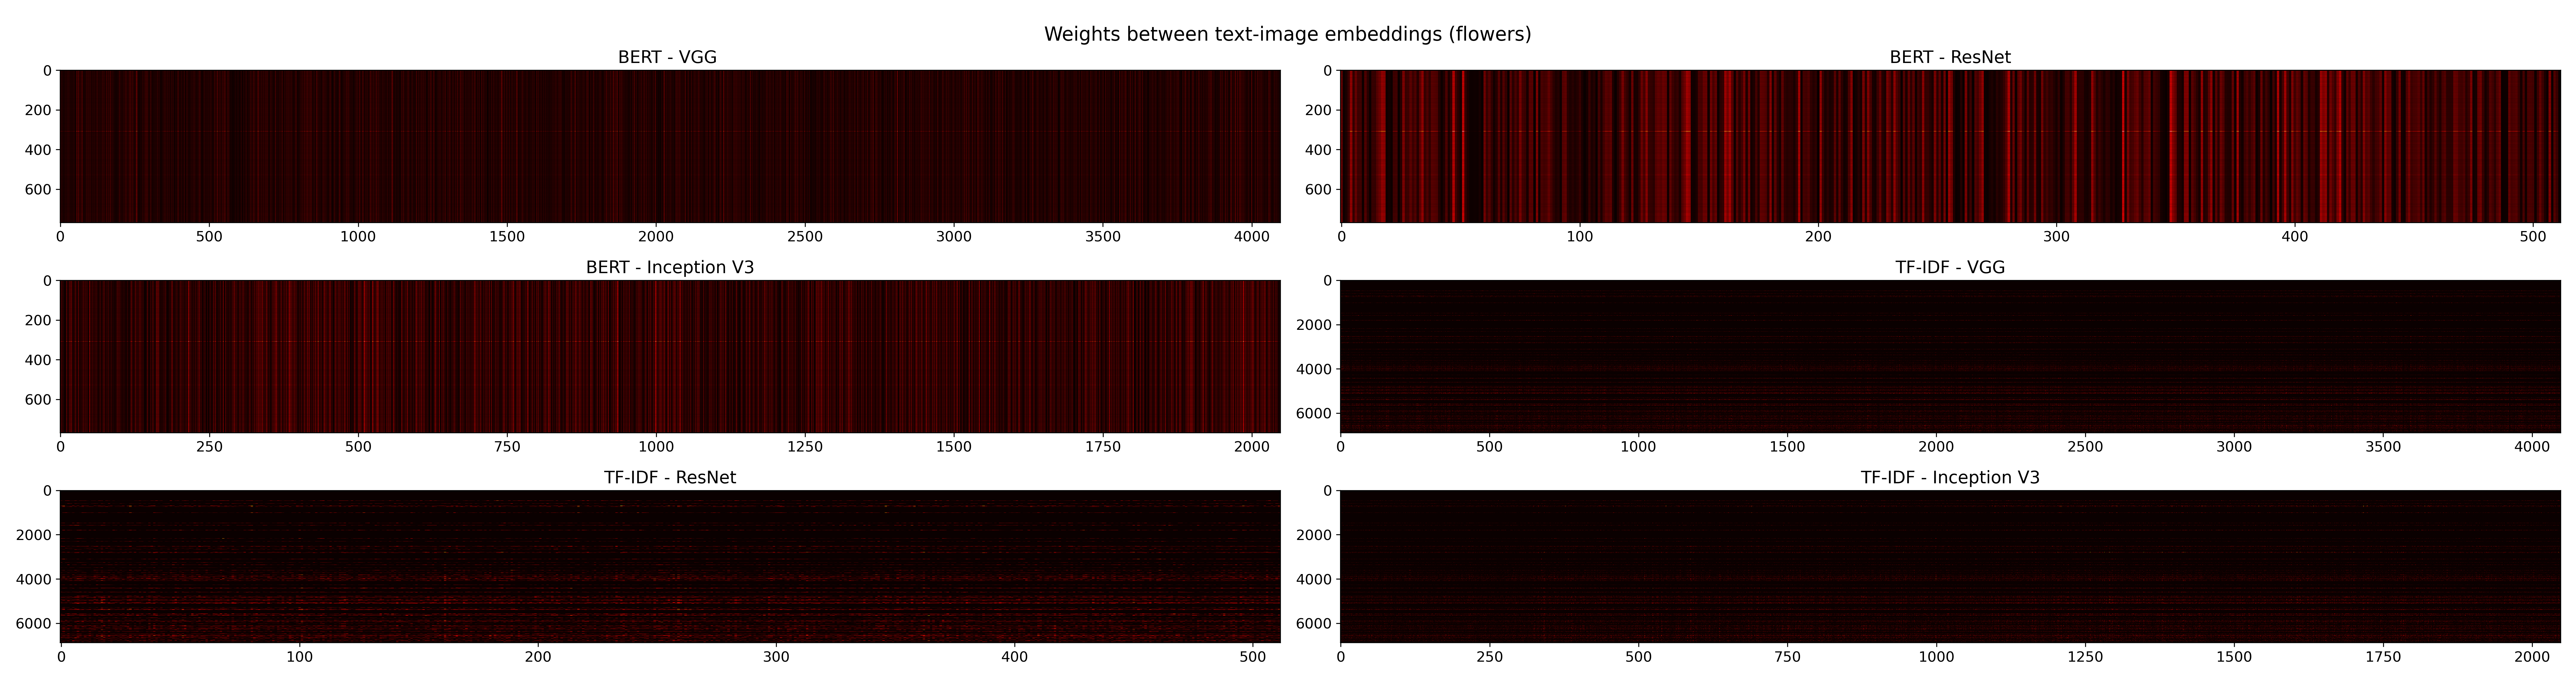
\includegraphics[width=1.1 \paperwidth]{figures/flowers-weights.png}
  \end{tabular}}% measure width
  \rotatebox{90}{\begin{minipage}[c][\textwidth][c]{\wd0}
    \usebox0
     \caption{The absolute value of the weights of the linear layer mapping the text embeddings into predicted image embeddings for each of the six presented models. The y-axis shows the components of the encoded text while the x-axis corresponds to the dimensions of the image embedding space.}
     \label{fig:weights}
  \end{minipage}}
\end{figure*}

In order to further understand the difference that the choice of text encoder makes, let us look at Figure \ref{fig:bert-top} and \ref{fig:tfidf-top}. The higher quality of the pairs with DistilBERT is not at all surprising when looking at Figure \ref{fig:bert-top}: most dimensions highly-correlate with at least one dimension of the other network. However, the hotspots on both sides leads us to believe that some dimensions have noticeably higher discriminative power than others. On the other hand, the components of TF-IDF require a multitude of image vector components to express, hence, the branching out nature of the connections going from left to right. Also, many tokens just do not end up with large weights, which means that these setups are less democratic and that may lead to less generalisability \cite{jegou2014triangulation}.
